\documentclass[12pt]{article}
\usepackage[left=1cm, right=1cm, top=2cm,bottom=1.5cm]{geometry} 

\usepackage[parfill]{parskip}
\usepackage[utf8]{inputenc}
\usepackage[T2A]{fontenc}
\usepackage[russian]{babel}
\usepackage{enumitem}
\usepackage[normalem]{ulem}
\usepackage{amsfonts, amsmath, amsthm, amssymb, mathtools,xcolor,accents}
\usepackage{blkarray}

\usepackage{tabularx}
\usepackage{hhline}

\usepackage{accents}
\usepackage{fancyhdr}
\pagestyle{fancy}
\renewcommand{\headrulewidth}{1.5pt}
\renewcommand{\footrulewidth}{1pt}

\usepackage{graphicx}
\usepackage[figurename=Рис.]{caption}
\usepackage{subcaption}
\usepackage{float}

%%Наименование папки откуда забирать изображения
\graphicspath{ {./images/} }

%%Изменение формата для ввода доказательства
\renewcommand{\proofname}{$\square$  \nopunct}
\renewcommand\qedsymbol{$\blacksquare$}

%%Изменение отступа на таблицах
\addto\captionsrussian{%
	\renewcommand{\proofname}{$\square$ \nopunct}%
}
%% Римские цифры
\newcommand{\RN}[1]{%
	\textup{\uppercase\expandafter{\romannumeral#1}}%
}

%% Для удобства записи
\newcommand{\MR}{\mathbb{R}}
\newcommand{\MC}{\mathbb{C}}
\newcommand{\MQ}{\mathbb{Q}}
\newcommand{\MN}{\mathbb{N}}
\newcommand{\MZ}{\mathbb{Z}}
\newcommand{\MTB}{\mathbb{T}}
\newcommand{\MTI}{\mathbb{I}}
\newcommand{\MI}{\mathrm{I}}
\newcommand{\MCI}{\mathcal{I}}
\newcommand{\MJ}{\mathrm{J}}
\newcommand{\MH}{\mathrm{H}}
\newcommand{\MT}{\mathrm{T}}
\newcommand{\MU}{\mathcal{U}}
\newcommand{\MV}{\mathcal{V}}
\newcommand{\MB}{\mathcal{B}}
\newcommand{\MF}{\mathcal{F}}
\newcommand{\MW}{\mathcal{W}}
\newcommand{\ML}{\mathcal{L}}
\newcommand{\MP}{\mathcal{P}}
\newcommand{\VN}{\varnothing}
\newcommand{\VE}{\varepsilon}
\newcommand{\dx}{\, dx}
\newcommand{\dy}{\, dy}
\newcommand{\dz}{\, dz}
\newcommand{\dd}{\, d}


\theoremstyle{definition}
\newtheorem{defn}{Опр:}
\newtheorem{rem}{Rm:}
\newtheorem{prop}{Утв.}
\newtheorem{exrc}{Упр.}
\newtheorem{problem}{Задача}
\newtheorem{lemma}{Лемма}
\newtheorem{theorem}{Теорема}
\newtheorem{corollary}{Следствие}

\newenvironment{cusdefn}[1]
{\renewcommand\thedefn{#1}\defn}
{\enddefn}

\DeclareRobustCommand{\divby}{%
	\mathrel{\text{\vbox{\baselineskip.65ex\lineskiplimit0pt\hbox{.}\hbox{.}\hbox{.}}}}%
}
\DeclareRobustCommand{\ndivby}{\mkern-1mu\not\mathrel{\mkern4.5mu\divby}\mkern1mu}


%Короткий минус
\DeclareMathSymbol{\SMN}{\mathbin}{AMSa}{"39}
%Длинная шапка
\newcommand{\overbar}[1]{\mkern 1.5mu\overline{\mkern-1.5mu#1\mkern-1.5mu}\mkern 1.5mu}
%Функция знака
\DeclareMathOperator{\sgn}{sgn}

%Функция ранга
\DeclareMathOperator{\rk}{\text{rk}}
\DeclareMathOperator{\diam}{\text{diam}}


%Обозначение константы
\DeclareMathOperator{\const}{\text{const}}

\DeclareMathOperator{\codim}{\text{codim}}

\DeclareMathOperator*{\dsum}{\displaystyle\sum}
\newcommand{\ddsum}[2]{\displaystyle\sum\limits_{#1}^{#2}}
\newcommand{\ddssum}[2]{\displaystyle\smashoperator{\sum\limits_{#1}^{#2}}}
\newcommand{\ddlsum}[2]{\displaystyle\smashoperator[l]{\sum\limits_{#1}^{#2}}}
\newcommand{\ddrsum}[2]{\displaystyle\smashoperator[r]{\sum\limits_{#1}^{#2}}}

%Интеграл в большом формате
\DeclareMathOperator{\dint}{\displaystyle\int}
\newcommand{\ddint}[2]{\displaystyle\int\limits_{#1}^{#2}}
\newcommand{\ssum}[1]{\displaystyle \sum\limits_{n=1}^{\infty}{#1}_n}

\newcommand{\smallerrel}[1]{\mathrel{\mathpalette\smallerrelaux{#1}}}
\newcommand{\smallerrelaux}[2]{\raisebox{.1ex}{\scalebox{.75}{$#1#2$}}}

\newcommand{\smallin}{\smallerrel{\in}}
\newcommand{\smallnotin}{\smallerrel{\notin}}

\newcommand*{\medcap}{\mathbin{\scalebox{1.25}{\ensuremath{\cap}}}}%
\newcommand*{\medcup}{\mathbin{\scalebox{1.25}{\ensuremath{\cup}}}}%

\makeatletter
\newcommand{\vast}{\bBigg@{3.5}}
\newcommand{\Vast}{\bBigg@{5}}
\makeatother

%Промежуточное значение для sup\inf, поскольку они имеют разную высоту
\newcommand{\newsup}{\mathop{\smash{\mathrm{sup}}}}
\newcommand{\newinf}{\mathop{\mathrm{inf}\vphantom{\mathrm{sup}}}}

%Скалярное произведение
\newcommand{\inner}[2]{\left\langle #1, #2 \right\rangle }
\newcommand{\linsp}[1]{\left\langle #1 \right\rangle }
\newcommand{\linmer}[2]{\left\langle #1 \vert #2\right\rangle }

%Подпись символов снизу
\newcommand{\ubar}[1]{\underaccent{\bar}{#1}}

%%Шапка для букв сверху
\newcommand{\wte}[1]{\widetilde{#1}}
\newcommand{\wht}[1]{\widehat{#1}}
\newcommand{\ovl}[1]{\overline{#1}}


%%Трансформация Фурье
\newcommand{\fourt}[1]{\mathcal{F}\left(#1\right)}
\newcommand{\ifourt}[1]{\mathcal{F}^{-1}\left(#1\right)}

%%Символ вектора
\newcommand{\vecm}[1]{\overrightarrow{#1\,}}

%%Пространстов матриц
\newcommand{\matsq}[1]{\operatorname{Mat}_{#1}}
\newcommand{\mat}[2]{\operatorname{Mat}_{#1, #2}}

%Оператор для действ и мнимых чисел
\DeclareMathOperator{\IM}{\operatorname{Im}}
\DeclareMathOperator{\RE}{\operatorname{Re}}
\DeclareMathOperator{\li}{\operatorname{li}}
\DeclareMathOperator{\GL}{\operatorname{GL}}
\DeclareMathOperator{\SL}{\operatorname{SL}}
\DeclareMathOperator{\Char}{\operatorname{char}}
\DeclareMathOperator\Arg{Arg}
\DeclareMathOperator\ord{ord}

%Оператор для образа
\DeclareMathOperator{\Ima}{Im}

%Делимость чисел
\newcommand{\modn}[3]{#1 \equiv #2 \; (\bmod \; #3)}
\newcommand{\nmodn}[3]{#1 \not\equiv #2 \; (\bmod \; #3)}

%%Взятие в скобки, модули и норму
\newcommand{\parfit}[1]{\left( #1 \right)}
\newcommand{\modfit}[1]{\left| #1 \right|}
\newcommand{\sqparfit}[1]{\left\{ #1 \right\}}
\newcommand{\normfit}[1]{\left\| #1 \right\|}

%%Функция для обозначения равномерной сходимости по множеству
\newcommand{\uconv}[1]{\overset{#1}{\rightrightarrows}}
\newcommand{\uconvm}[2]{\overset{#1}{\underset{#2}{\rightrightarrows}}}

%% Функция для добавления круга сверху множества
\newcommand{\Circ}[1]{\accentset{\circ}{#1}}

%%Функция для обозначения нижнего и верхнего интегралов
\def\upint{\mathchoice%
	{\mkern13mu\overline{\vphantom{\intop}\mkern7mu}\mkern-20mu}%
	{\mkern7mu\overline{\vphantom{\intop}\mkern7mu}\mkern-14mu}%
	{\mkern7mu\overline{\vphantom{\intop}\mkern7mu}\mkern-14mu}%
	{\mkern7mu\overline{\vphantom{\intop}\mkern7mu}\mkern-14mu}%
	\int}
\def\lowint{\mkern3mu\underline{\vphantom{\intop}\mkern7mu}\mkern-10mu\int}

%%След матрицы
\DeclareMathOperator*{\tr}{tr}

\makeatletter
\renewcommand*\env@matrix[1][*\c@MaxMatrixCols c]{%
	\hskip -\arraycolsep
	\let\@ifnextchar\new@ifnextchar
	\array{#1}}
\makeatother


%% Переопределение функции хи, чтобы выглядела более приятно
\makeatletter
\@ifdefinable\@latex@chi{\let\@latex@chi\chi}
\renewcommand*\chi{{\@latex@chi\smash[t]{\mathstrut}}} % want only bottom half of \mathstrut
\makeatletter

\setcounter{MaxMatrixCols}{20}

\begin{document}
\lhead{Математический анализ - \RN{4}}
\chead{Шапошников С.В.}
\rhead{Лекция - 5}

\section*{Интеграл Римана по множеству}

\begin{defn}
	\uwave{Интеграл Римана по произвольному множеству $E$} (где $E$ - ограничено) это интеграл: 
	$$
		\ddint{E}{} f(x)dx = \ddint{\MI}{} \wte{f}(x)dx, \quad \ovl{E}\subset \Circ{\MI}, \quad
		\wte{f}(x) = 
		\begin{cases}
			f(x), & x \in E \\
			0, & x \not\in E
		\end{cases}
	$$
\end{defn}
\begin{rem}
	Можно себе представлять, что все функции определены всюду и мы берём: $\wte{f}(x) = f(x){\cdot}\chi_E(x)$.
\end{rem}
Как мы проверели, определение - корректно.
\begin{prop}
	$\int_E 1dx$ существует $\Leftrightarrow \partial E$ - множество меры нуль по Лебегу.
\end{prop}
\begin{defn}
	Множество $E$ \uwave{допустимо} (\uwave{измеримо по Жордану}), если $E$ - ограничено и $\partial E$ это множество меры нуль по Лебегу.
\end{defn}
\begin{defn}
	\uwave{Объемом допустимого множества $E$} называется интеграл: $|E| = \int_{E} 1 dx$.
\end{defn}
\begin{prop}
	Если $E$ допустимо и $|E| = 0$, то $\forall$ ограниченная функция $f$ интегрируема по Риману на $E$ и кроме того, верно: $\int_{E}f(x)dx = 0$.
\end{prop}
\begin{theorem}(\textbf{Критерий Лебега для допустимых множеств})
	Пусть $E$ - допустимое множество. Тогда $f$ интегрируема на $E \Leftrightarrow f$ - ограничена на $E$ и непрерывна почти всюду на $E$.
\end{theorem}
\begin{prop}
	Если $E$ это компакт меры нуль по Лебегу, то $E$ - допустимое множество и $|E| = 0$.
\end{prop}
\begin{proof}
	Поскольку $E$ - компакт, то $\partial E \subset E \Rightarrow \partial E$ это множество меры нуль $\Rightarrow \chi_E(x)$ - интегрируема и почти всюду равна $0 \Rightarrow |E| = 0$ (см. утв. $6$ лекция $3$).
\end{proof}

\begin{rem}
	Из того, что ограниченное множество является множеством меры нуль не следует, что это множество - допустимое.
\end{rem}
\textbf{Пример}: $\MQ$ в отрезке $[0,1]$.

\begin{exrc}
	Верно ли, что всякий компакт является допустимым множеством? (ответ - нет, но нужно понять может ли у компакта граница быть не меры $0$).
\end{exrc}

\begin{prop}
	Если $E_1$ и $E_2$ - допустимые множества, то $E_1 \cup E_2, \, E_1 \setminus E_2, \, E_1 \cap E_2$ - допустимые множества.
\end{prop}
\begin{rem}
	Таким образом, $\mathcal{A} = \{E \subset \MI \mid E \text{ - допустимые }\}$ - алгебра подмножеств в $\MI$. Является ли это $\sigma$-алгеброй? Нет, пример: объединение рациональных точек (то есть с рациональными координатами), так как точка - допустимое множество, а счётное объединение точек уже может быть не допустимым.
\end{rem}
\begin{proof}
	Ограниченность - очевидна: объединение, пересечение, вычитание ограниченных множеств - ограниченно. Покажем, что: $\partial (E_1 \cup E_2), \, \partial(E_1 \cap E_2), \, \partial (E_1 \setminus E_2) \subset \partial E_1 \cup \partial E_2$. Пусть $a\not\in \partial E_1 \cup \partial E_2$, тогда возможно несколько вариантов:
	\begin{enumerate}[label=\arabic*)]
		\item $a$ - внешняя для $E_1$ и для $E_2 \Rightarrow E_1 \cup E_2$ - внешняя, $E_1 \cap E_2$ - внешняя, $E_1 \setminus E_2$ - внешняя $\Rightarrow a$ не является граничной;
		\item $a$ - внешняя для $E_1$ и внутренняя для $E_2 \Rightarrow E_1 \cup E_2$ - внутренняя, $E_1 \cap E_2$ - внешняя (есть окрестность, где нет точек $E_1$), $E_1 \setminus E_2$ - внешняя $\Rightarrow a$ не является граничной;
		\item $a$ - внутренняя для $E_1$ и внешняя для $E_2 \Rightarrow E_1 \cup E_2$ - внутренняя, $E_1 \cap E_2$ - внешняя (есть окрестность, где нет точек $E_2$), $E_1 \setminus E_2$ - внутренняя $\Rightarrow a$ не является граничной;
		\item $a$ - внутренняя для $E_1$ и для $E_2 \Rightarrow E_1 \cup E_2$ - внутренняя, $E_1 \cap E_2$ - внутренняя, $E_1 \setminus E_2$ - внешняя (есть окрестность, где все точки из $E_2 \Rightarrow$ не из дополнения) $\Rightarrow a$ не является граничной;
	\end{enumerate}
	Следовательно, все эти множества входят в $\partial E_1 \cup \partial E_2$, а объединение двух множеств меры нуль это множество меры нуль.
\end{proof}

\section*{Свойства интеграла Римана по множеству}
\begin{theorem}
	Пусть $E$ - допустимое множество (в пунктах $1-2$ допустимость не требуется).
	\begin{enumerate}[label=\arabic*)]
		\item Если $f,g$ интегрируемы на $E$, то $\forall \alpha,\beta \in \MR$, $\alpha{\cdot}f(x) + \beta{\cdot}g(x)$ интегрируемы на $E$ и верно:
		$$
			\ddint{E}{}(\alpha{\cdot}f(x) + \beta{\cdot}g(x)) dx = \alpha \ddint{E}{}f(x)dx + \beta \ddint{E}{}g(x)dx
		$$ 
		\item Если $f,g$ интегрируемы на $E$ и $f \leq g$, то:
		$$
			\ddint{E}{}f(x)dx \leq \ddint{E}{}g(x)dx
		$$
		\item (\textbf{Теорема о среднем}): Если $f$ интегрируема на $E$, то $\exists \, \mu \in [\inf\limits_{E}f, \sup\limits_{E}f]$ такое, что:
		$$
			\ddint{E}{}f(x)dx = \mu{\cdot}|E|
		$$
		Если $E$ - связно и $f$ - непрерывна на $E$, то $\exists \, c \in E \colon \mu = f(c)$;
		\item (\textbf{Полезные неравенства}): Пусть $f,g$ интегрируемы на $E$, тогда:
		$$
			\left| \ddint{E}{}f(x)dx \right| \leq \ddint{E}{}|f(x)|dx, \quad \ddint{E}{}f(x){\cdot}g(x)dx \leq \sqrt{\ddint{E}{}f^2(x)dx}{\cdot}\sqrt{\ddint{E}{}g(x)dx}
		$$
	\end{enumerate}
\end{theorem}
\begin{proof}\hfill
	\begin{enumerate}[label=\arabic*)]
		\item $f,g$ интегрируемы на $E$, тогда по определению: $\exists \, \MI \colon \ovl{E} \subset \Circ{\MI}$, рассматриваем $\wte{f}$ и $\wte{g}$:
		$$
			\ddint{E}{}\alpha{\cdot}f(x) + \beta{\cdot}g(x)dx = \ddint{\MI}{}\alpha{\cdot}\wte{f}(x) + \beta{\cdot}\wte{g}(x)dx =  
		$$
		$$
			= \alpha{\cdot}\ddint{\MI}{}\wte{f}(x)dx + \beta{\cdot}\ddint{\MI}{}\wte{g}(x)dx = \alpha{\cdot} \ddint{E}{}f(x)dx + \beta {\cdot}\ddint{E}{}g(x)dx
		$$
		Существование этих интегралов это ровно существование интегралов от $\wte{f}$ и $\wte{g}$ по какому-либо брусу, содержащему $\ovl{E}$;
		\item  $f,g$ интегрируемы на $E$, тогда по определению: $\exists \, \MI \colon \ovl{E} \subset \Circ{\MI}$, рассматриваем $\wte{f}$ и $\wte{g}$:
		$$
			f\leq g \Rightarrow \wte{f} \leq \wte{g} \Rightarrow \ddint{E}{}f(x)dx =  \ddint{\MI}{}\wte{f}(x)dx \leq \ddint{\MI}{}\wte{g}(x)dx = \ddint{E}{}g(x)dx
		$$
		\item $f$ - интегрируема $\Rightarrow f$ - ограничена $\Rightarrow \inf\limits_E f \leq f \leq \sup\limits_E f$, поскольку $E$ - допустимое, то:
		$$
			\inf\limits_E f(x){\cdot}|E| \leq \ddint{E}{}f(x)dx \leq  \sup\limits_E f(x){\cdot}|E|
		$$
		Если $|E| = 0$, то $\int_E f(x)dx = 0 \Rightarrow \mu \in \MR$ - произвольное. Если $|E| \neq 0$, то:
		$$
			\inf\limits_E f(x) \leq \dfrac{1}{|E|}{\cdot}\ddint{E}{}f(x)dx \leq  \sup\limits_E f(x) \Rightarrow \mu \coloneqq \dfrac{1}{|E|}{\cdot}\ddint{E}{}f(x)dx \in [\inf\limits_{E}f, \sup\limits_{E}f]
		$$
		\item Заметим, что: $-|f(x)| \leq f(x) \leq |f(x)|$, тогда по интегрируемости и монотонности:
		$$
			-\ddint{E}{}|f(x)|dx \leq \ddint{E}{}f(x)dx \leq \ddint{E}{}|f(x)|dx \Rightarrow \left|\ddint{E}{}f(x)dx \right| \leq \ddint{E}{}|f(x)|dx
		$$
		$f,g$ интегрируемы на $E$, тогда по определению: $\exists \, \MI \colon \ovl{E} \subset \Circ{\MI}$ и $\wte{f}, \wte{g}$ интегрируемы на $\MI \Rightarrow \wte{f}{\cdot}\wte{g}$ интегрируемы на $\MI$, следовательно по определению $f{\cdot}g$ интегрируемы на $E$. По неравенству Коши-Буняковского для интегрируемых по Риману функций на $\MI$ будет верно: $|\langle\wte{f},\wte{g}\rangle| \leq \|\wte{f}\|{\cdot}\|\wte{g}\|$, тогда:
		$$
			\ddint{\MI}{}\wte{f}(x){\cdot}\wte{g}(x)dx = \ddint{E}{}f(x){\cdot}g(x)dx \leq \sqrt{\ddint{\MI}{}\wte{f}(x)dx}{\cdot}\sqrt{\ddint{\MI}{}\wte{g}(x)dx} = \sqrt{\ddint{E}{}f(x)dx}{\cdot}\sqrt{\ddint{E}{}g(x)dx}
		$$
	\end{enumerate}
\end{proof}

\begin{theorem}\hfill
	\begin{enumerate}[label =\arabic*)]
		\item Пусть $E$ - допустимое множество и $f$ интегрируема на $E$, если $D \subset E$ и $D$ - допустимо, то $f$ интегрируема на $D$;
		\item Если $E_1, E_2$ - допустимые и $f$ интегрируема на $E_1$ и на $E_2$, то $f$ интегрируема на $E_1 \cup E_2$ и верно:
		$$
			\ddint{E_1 \cup E_2}{} f(x)dx = \ddint{E_1}{}f(x)dx + \ddint{E_2}{}f(x)dx - \ddint{E_1 \cap E_2}{}f(x)dx
		$$
		В частности, если $|E_1 \cap E_2| = 0$, то последнего слагаемого нет:
		$$
			\ddint{E_1 \cup E_2}{} f(x)dx = \ddint{E_1}{}f(x)dx + \ddint{E_2}{}f(x)dx
		$$
	\end{enumerate}
\end{theorem}
\begin{rem}
	Заметим, что в первом пункте если отказаться от допустимости $D$, то утверждение станет не верным. Например, $1$ интегрируема на отрезке, но не является интегрируемой по Риману на $\MQ$.
\end{rem}
\begin{proof}\hfill
	\begin{enumerate}[label=\arabic*)]
		\item $f$ интегрируема на $E \Rightarrow$ по критерию Лебега $f$ ограничена на $E \Rightarrow f$ ограничена на $D$. Если точка $x$ - точка разрыва $f$ на множестве $D$, то $x$ - точка разрыва $f$ на множестве $E \Rightarrow$ множество точек разрыва $f$ на $D \subset$ множество точек разрыва $f$ на $E \Rightarrow$ это точки множества меры нуль $\Rightarrow$ по критерию Лебега $f$ интегрируема на $D$; 
		\item Пусть $\ovl{E}_1 \cup \ovl{E}_2 \subset \Circ{\MI}$ и считаем, что $f$ определена на $\MI$ (как угодно продолжаем её вне $\ovl{E}_1 \cup \ovl{E}_2$). Очевидно равенство:
		$$
			f{\cdot}\chi_{E_1\cup E_2} = f{\cdot}\chi_{E_1} + f{\cdot}\chi_{E_2} - f{\cdot}\chi_{E_1 \cap E_2}
		$$
		Тогда, $f$ интегрируема на $\MI \Rightarrow f{\cdot}\chi_{E_1}$ - интегрируемаая функция на $\MI$, аналогично можно сказать про $f{\cdot}\chi_{E_2}$ - она интегрируема на $\MI$. Взяли подмножество: $E_1 \cap E_2 \subset E_1 \Rightarrow$ оно допустимое $\Rightarrow  f{\cdot}\chi_{E_1 \cap E_2}$ интегрируема на $\MI$ (смотри первый пункт). По линейности, сумма интегрируемых функций даст интегрируему функцию $\Rightarrow f$ интегрируема на $E_1 \cup E_2$. Применяем линейность и получаем:
		$$
			\ddint{\MI}{}f(x){\cdot}\chi_{E_1 \cup E_2}(x)dx = \ddint{\MI}{}f(x){\cdot}\chi_{E_1}(x)dx + \ddint{\MI}{}f(x){\cdot}\chi_{E_2}(x)dx - \ddint{\MI}{}f(x){\cdot}\chi_{E_1 \cap E_2}(x)dx
		$$
	\end{enumerate}
\end{proof}
\begin{rem}
	То есть на самом деле аддитивности, как отдельного свойства, на самом деле нет. Аддитивность это следствие линейности, применяемой с индикаторами.
\end{rem}

\begin{theorem}(\textbf{Фубини})
	Пусть $E$ - допустимое множество, $\ovl{E} \subset \Circ{\MI}$ и $\MI = \MI_x \times \MI_y$, где $\MI_x \subset \MR^n,\, \MI_y \subset \MR^m$.
	\begin{figure}[H]
		\centering
		\includegraphics[width=0.35\textwidth]{MA4L5_1.eps}
		\caption{Множество $E_x$.}
		\label{5_1}
	\end{figure}
	Положим $E_x= \{y \mid (x,y) \subset E\} \subset \MI_y$. Пусть $\forall x \in \MI_x,\, E_x$ - допустимое в $\MR^m$, функция $f \colon E \to \MR$ интегрируема по Риману и $\forall x, \, y \mapsto f(x,y)$ интегрируема на $E_x$. Тогда верно:
	$$
		\iint_E f(x,y)dxdy = \ddint{\MI_x}{}\left(\; \ddint{E_x}{}f(x,y)dy\right)dx
	$$
\end{theorem}
\begin{proof}
	Рассмотрим индикатор множества $E$ и заметим, что: $\chi_E(x,y) = \chi_{E_x}(y)$, поскольку оно верно при каждом фиксированном $x$ для всех $y \Rightarrow$ выполнено вообще для всех $(x,y) \Rightarrow$ равенство верно. Считаем, что $f$ продолжена на весь брус $\MI$ вне множества $E$, по условию функция $y \mapsto f(x,y)\chi_{E_x}(y)$ интегрируема на $\MI_y$. Тогда, как вся функция: $f(x,y){\cdot}\chi_E(x,y) = f(x,y){\cdot}\chi_{E_x}(y)$ интегрируема на $\MI$. По теореме Фубини для бруса мы получаем:
	$$
		\iint_E f(x,y)dxdy = \iint_{\MI}f(x,y)\chi_{E}(x,y)dxdy = \ddint{\MI_x}{}\left( \;\ddint{\MI_y}{}f(x,y){\cdot}\chi_{E_x}(y)dy\right)dx = \ddint{\MI_x}{}\left( \; \ddint{E_x}{}f(x,y) dy\right)dx
	$$
	где последнее верно по определению.
\end{proof}
\begin{rem}
	От допустимости можно отказаться, но пришлось бы давать такие же комментарии, как мы давали в теореме Фубини. Более того, можно было бы не требовать допустимости $E_x$, а требовать только интегрируемость $f$ на $E_x$, также как можно было бы не требовать допустимость $E$, а требовать интегрируемость $f$ на $E$.
\end{rem}
\begin{corollary}(\textbf{Принцип Кавальери})
	$$
		|E| = \ddint{\MI_x}{}|E_x|dx
	$$
\end{corollary}
\begin{rem}
	Значение принципа следующее: если вы хотите найти объем какого-то тела, то вы начинаете его рассекать, смотреть сечения и потом, грубо говоря, суммировать площади сечения.
	\begin{figure}[H]
		\centering
		\includegraphics[width=0.35\textwidth]{MA4L5_2.eps}
		\caption{Разбиение на сечения и получение объема тела $E$.}
		\label{5_2}
	\end{figure}
\end{rem}
\begin{rem}
	Отсюда возможны простые наблюдения: если взяли два тела над одним и тем же множеством (например, отрезком, квадратом) и начинаем измерять, что площади сечения совпадают $\Rightarrow$ объемы совпадают. И опять же это будет следовать из формулы принципа Кавальери $\Rightarrow V_1 = V_2$.
	\begin{figure}[H]
		\centering
		\includegraphics[width=0.35\textwidth]{MA4L5_3.eps}
		\caption{Совпадение объемов у тел с совпадающими сечениями.}
		\label{5_3}
	\end{figure}
\end{rem}

\begin{exrc}
	Найти объем шара с помощью объема цилиндра и конуса.
\end{exrc}
\begin{proof}
	Пусть у нас есть шар радиуса $a$, площадь его сечения на расстоянии от центра $h$ равна:
	$$
		S_{sec}^{sph} = \pi{\cdot}\left(\sqrt{a^2 - h^2}\right)^2 = \pi{\cdot}(a^2 - h^2)
	$$
	Площадь сечения цилиндра радиуса $a$ в любой точке равна:
	$$
		S_{sec}^{cyl} = \pi{\cdot}a^2
	$$
	Площадь сечения двойного конуса радиуса $a$, вписанного в цилиндр высоты $a$ на расстоянии $h$ от центра равна:
	$$
		S_{sec}^{con} = \pi{\cdot}h^2
	$$
	Таким образом, разность площадей цилиндра и конуса на расстоянии $h$ от центра конуса равна:
	$$
		S_{sec}^{cyl} - S_{sec}^{con} = \pi{\cdot}a^2 - \pi{\cdot}h^2 = \pi{\cdot}(a^2 - h^2) = S_{sec}^{sph}
	$$
	Тогда по принципу Кавальери, объем шара, равен объему цилиндра радиуса $a$ и высотой $2a$ за вычетом объема двойного конуса радиуса $a$ и высотой $2a$.
	\begin{figure}[H]
		\centering
		\includegraphics[width=0.55\textwidth]{MA4L5_4.eps}
		\caption{Площади сечения шара, цилиндра и конуса.}
		\label{5_4}
	\end{figure}
\end{proof}
\newpage
\section*{Формула заменых переменных}
\begin{prop}
	Пусть $\MU$ - открытое множество в $\MR^n$, тогда:
	\begin{enumerate}[label=\arabic*)]
		\item $\MU$ - это объединение не более, чем счётного набора замкнутых кубов, которые пересекаются лишь по границе;
		\item $\MU$ - это объединение не более, чем счётного набора замкнутых кубов, которые попарно не пересекаются и множества меры нуль по Лебегу;
		\item $\MU$ - это объединение не более, чем счётного набора замкнутых шаров положительного радиуса, которые попарно не пересекаются и множества меры нуль по Лебегу;
	\end{enumerate}
\end{prop}
\begin{proof}\hfill
	\begin{enumerate}[label=\arabic*)]
		\item Пройдем все оси с шагом $1\Rightarrow$ появляется сетка, те клетки которые целиком попали в $\MU$, мы забираем. И говорим, что $F_1$ - набор всех клеток с ребром $1$, попавших в $\MU$:
		\begin{figure}[H]
			\centering
			\includegraphics[width=0.35\textwidth]{MA4L5_5.eps}
			\caption{Построение множества $F_1$.}
			\label{5_5}
		\end{figure}
		Дальше мы идем с шагом $\tfrac{1}{2}$ по тем же самым осям, появляются новые клетки, которые мы могли не взять с ребром $\tfrac{1}{2}$. И говорим, что $F_{\frac{1}{2}}$ - набор всех клеток с ребром $\tfrac{1}{2}$, попавших в $\MU$, но которые не лежат в уже взятых.
		\begin{figure}[H]
			\centering
			\includegraphics[width=0.35\textwidth]{MA4L5_6.eps}
			\caption{Построение множества $F_{\frac{1}{2}}$.}
			\label{5_6}
		\end{figure}
		И так далее, продолжаем формировать множества $F_{\frac{1}{4}}, F_{\frac{1}{8}}, F_{\frac{1}{16}}, \dotsc$. Таким образом, мы получаем большое множество из этих клеток, пусть $\{K_m\}$ это все клетки всех $F_{\frac{1}{2^p}}$. По построению ясно, что никакие две не пересекаются внутренностями:
		$$
			\forall k,l, k \neq l,\,  \Circ{K}_k \cap \Circ{K}_l = \VN, \, K_k \cap K_l \subset \partial K_k \cup \partial K_l 
		$$
		Нам необходимо проверить, что: $\MU = \cup_m K_m$. Возьмем произвольную точку $a \in \MU \Rightarrow$ нам необходимо проверить, что $\exists \, l \colon a \in K_l$. Поскольку $\MU$ - открыто, то $a$ лежит в нем вместе с некоторой своей окрестностью, пусть это будет брус $\MI_a$. Далее, делаем разбиение осей длины меньше, чем расстояние от точки $a$ до краев этого бруса. То есть:
		$$
			\MI_a = [\alpha_1,\beta_1]\times[\alpha_2,\beta_2]\times \dotsc \times [\alpha_n, \beta_n] \Rightarrow \exists \, r \colon \dfrac{1}{2^r} < \beta_i - \alpha_i, \, \forall i = \ovl{1,n}
		$$
		Таким образом, каждая из координат $a = (a_1,\dotsc, a_n)$ попадет в какой-то из отрезков разделения осей $\Rightarrow$ вся точка попадет в квадрат, который должен быть построен на $r$-ом шаге. И либо этот квадрат уже лежит в каком-то квадрате, который мы взяли раньше $\Rightarrow$ точка $a$ лежит в каком-то квадрате, взятом раньше, либо в квадрате на $r$-ом шаге $\Rightarrow$ точка $a$ лежит в каком-то квадрате.
		\begin{figure}[H]
			\centering
			\includegraphics[width=0.3\textwidth]{MA4L5_7.eps}
			\caption{Нахождение квадрата для любой точки $a \in \MU$.}
			\label{5_7}
		\end{figure}
		Квадраты могут пересекаться лишь по границам $\Rightarrow \MU = \bigcup\limits_m K_m$;
		\item \textbf{\uline{Идея доказательства}}: Квадраты, построенные на предыдущем шаге могут пересекаться по границам $\Rightarrow$ нужно границы удалить $\Rightarrow$ объединение границ будет образовывать множество меры нуль. Теперь у нас есть множество попарно непересекающихся открытых квадратов. 
		\begin{figure}[H]
			\centering
			\includegraphics[width=0.3\textwidth]{MA4L5_8.eps}
			\caption{Выделение замкнутого куба внутри открытого квадрата.}
			\label{5_8}
		\end{figure}
		Каждый из таких квадратов теперь надо представить в виде объединения замкнутых кубов. Для этого, мы берем число $q \in (0,1)$ и вырезаем на каждом ребре длины $l$ центрированный отрезок длины $ql \Rightarrow$ вырезается замкнутый квадрат. Если объем исходного квадрата был $|K|$, то объем вырезанного будет $q^n|K|$. После этого, весь квадрат распадается в объединении брусков. Их можно также раздробить на квадраты, и затем для каждого из них повторить процедуру.
		\begin{figure}[H]
			\centering
			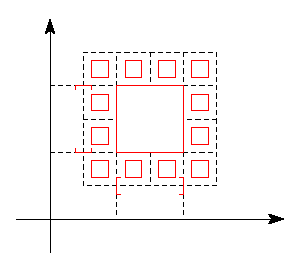
\includegraphics[width=0.3\textwidth]{MA4L5_9.eps}
			\caption{Повторение процедуры разбинеия.}
			\label{5_9}
		\end{figure}
		Следовательно, надо подобрать $q$ так, чтобы сумма объемов в итоге сходилась к $|K|$. То что осталось вне - множестве меры нуль (решение не полное) -упр. Получится, что квадрат это объединение замкнутых попарно непересекающихся кубов;
		\item Упр. Аналогично, должно разбираться на действительном анализе.
	\end{enumerate}
\end{proof}

\begin{prop}
	В определении множества меры нуль по Лебегу произвольные бруски можно заменить кубами.
\end{prop}
\begin{proof}
	По определению:
	$$
		\forall \VE > 0, \, \exists\, \{\MI_m\} \colon E \subset \bigcup\limits_m\MI_m \wedge \ddsum{m}{}|\MI_m| < \VE
	$$
	\begin{enumerate}[label=\arabic*)]
		\item Можно в определении брать бруски с рёбрами, рациональной длины: имеющийся брусок можно поместить в брусок у которого рёбра удлинились максимум в три раза. 
		\begin{figure}[H]
			\centering
			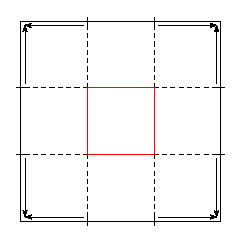
\includegraphics[width=0.2\textwidth]{MA4L5_10.eps}
			\caption{Повторение процедуры разбиения.}
			\label{5_10}
		\end{figure}
		Объем нового бруска $\wte{\MI}$ будет ограничен:
		$$
			|\wte{\MI}| \leq 3^n|\MI|
		$$
		Тогда рациональные точки найдутся в удлиненных ребрах $\Rightarrow$ берём ребро рациональной длины.
		\begin{figure}[H]
			\centering
			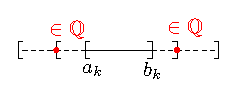
\includegraphics[width=0.25\textwidth]{MA4L5_11.eps}
			\caption{Взятие ребра рациональной длины.}
			\label{5_11}
		\end{figure} 
		Увеличение объема обходится нам в одну фиксированную константу, если $\VE > 0$ - произвольное, то мы ничего не теряем;
		\item Бруски с рёбрами рациональной длины гораздо проще разбивается на кубы. Например, если у нас брусок $K_j^m$ с рёбрами $\tfrac{k}{l}$ и $\tfrac{p}{q}$, тогда можно разбить такой прямоугольник на квадраты, взяв дробление каждой стороны с шагом: $\tfrac{1}{lq}$. 
		\begin{figure}[H]
			\centering
			\includegraphics[width=0.2\textwidth]{MA4L5_12.eps}
			\caption{Разбиение бруска на кубы.}
			\label{5_12}
		\end{figure} 
		Объем таких квадратов:
		$$
			\ddsum{j}{}|K_j^m| = |\MI_m|
		$$
		где $K_j^m$ будут кубами и вместе с этим верно: 
		$$
			E \subset \bigcup\limits_{j,m} K_j^m, \quad \sum_{j,m}|K_j^m| < \VE
		$$
	\end{enumerate}
\end{proof}

\begin{prop}
	Пусть $\MU$ - открытое множество $\subset \MR^n$, $f\colon \MU \to \MR^k, \, k \geq n$ - локально Липшицева, то есть 
	$$
		\forall\,  \MI \text{ - замкнутый брус } \subset \MU, \, \exists \, C(\MI) > 0 \colon \forall x,y \in \MI, \, \|f(x) - f(y)\| \leq C(\MI){\cdot}\|x -y \|
	$$
	Тогда для всякого множества $E \subset \MU$ меры нуль множество $f(E)$ является множеством меры нуль.
\end{prop}

\begin{rem}
	Если заменить $f$ на непрерывную, то это утверждение - не верно, даже для гомеоморфизма (можно построить пример с помощью Канторовского множества, что множество меры нуль Канторовское перешло в множество меры $\tfrac{1}{2}$).
\end{rem}

\end{document}